\documentclass[9pt]{beamer}
\usepackage[utf8]{inputenc}
\usetheme{Berkeley}
\setbeamertemplate{blocks}[rounded][shadow=true]
\usepackage{graphicx}
\usepackage{amsmath}
\usepackage{amssymb}
\usepackage{hyperref}
\usepackage{xcolor}
\usepackage{tikz}
\usetikzlibrary{tikzmark,positioning}

\makeatletter
\def\mathcolor#1#{\@mathcolor{#1}}
\def\@mathcolor#1#2#3{%
  \protect\leavevmode
  \begingroup
    \color#1{#2}#3%
  \endgroup
}
\makeatother

\definecolor{ForestGreen}{cmyk}{0.83,0.21,1,0.08}
\definecolor{ONTech-dark-blue}{cmyk}{1,0.58,0.09,0.46}
\definecolor{ONTech-light-blue}{cmyk}{1,0.31,0,0}
\definecolor{ONTech-orange}{cmyk}{0,0.70,1,0}
\definecolor{ONTech-warm-grey}{cmyk}{0.9,0.11,0.13,0.20}
\definecolor{ONTech-cool-grey}{cmyk}{0.20,0.14,0.12,0.40}
\definecolor{ONTech-dark-grey}{cmyk}{0.45,0.25,0.16,0.59}
\definecolor{ONTech-navy}{cmyk}{1,0.75,0.50,0.50}

% \renewcommand{\vec}[1]{\ensuremath{\boldsymbol{#1}}}
% \newcommand{\mtx}[1]{\ensuremath{\boldsymbol{#1}}}

\renewcommand{\vec}[1]{\ensuremath{\overline{#1}}}
\newcommand{\mtx}[1]{\ensuremath{\overline{\overline{#1}}}}
\newcommand{\vect}[1]{\ensuremath{\boldsymbol{#1}}}
 
%Information to be included in the title page:
\title{Reduced Order Modelling}
\subtitle{Exploring Reduced Basis Method Through Toy Problems}
\author{Parikshit Bajpai}
\date{MCSC 6020G - Numerical Analysis \\ \small{\today}}

% Add slide numbers in navigation bar
\addtobeamertemplate{navigation symbols}{}{%
    \usebeamerfont{footline}%
    \usebeamercolor[fg]{footline}%
    \hspace{1em}%
    \insertframenumber/\inserttotalframenumber
}
 

\begin{document}
 
\frame{\titlepage}

\frame{\tableofcontents} 

\section{Motivation and Objectives}
\begin{frame}{Motivation and Objective}
\centering
\textbf{The full order simulation is extremely costly!}

Can we reduce the computational time and cost associated with these simulations without compromising with the accuracy?

\vspace{1em}
\begin{alertblock}{Objective}
    \centering Demonstrate the principles and use of Reduced Basis Method for a heat conduction toy problem.
\end{alertblock}
\end{frame}

\section{Reduced Basis Method}
\begin{frame}{Solution Manifold}
    \begin{block}{Exact Solution}
        Find $u(\mu) \in \mathbb{V}$ such that
        $$\mathrm{a}(u(\mu), v; \mu) = \mathrm{f}(v;\mu) \mspace{20mu} \forall v \in \mathbb{V}$$
    \end{block}
    \begin{block}{Solution Manifold}
        $$\mathcal{M} = \{u(\mu)|\mu \in \mathbb{P}\} \subset \mathbb{V}$$
        where each $u(\mu) \in \mathbb{V}$ corresponds to the solution of exact problem.
    \end{block}
    \begin{exampleblock}{Truth Solution}
        Find $u_{\delta}(\mu) \in \mathbb{V}_{\delta}$ such that
        $$\mathrm{a}(u_{\delta}(\mu), v_{\delta}; \mu) = \mathrm{f}(v_{\delta};\mu) \mspace{20mu} \forall v_{\delta} \in \mathbb{V}_{\delta}$$
    \end{exampleblock}
    \begin{exampleblock}{Truth Manifold}
        $$\mathcal{M}_{\delta} = \{u_{\delta}(\mu)|\mu \in \mathbb{P}\} \subset \mathbb{V}_{\delta}$$
        where each $u_{\delta}(\mu) \in \mathbb{V}_{\delta}$ corresponds to the solution of exact problem.
    \end{exampleblock}
\end{frame}

\begin{frame}{Reduced Basis}
    \begin{block}{}
        Represent the truth solution based on $N$ dimensional subspace $\mathbb{V}_{rb}$ of $\mathbb{V}_{\delta}$, where $N \ll N_{\delta}$ and the reduced basis space is given by 
    $$ \mathbb{V}_{rb} = \mathrm{span}\{\xi_1,\dots,\xi_N\} \subset \mathbb{V}_{\delta}$$
    where, $\{\xi_n\}_{n=1}^{N} \subset \mathbb{V}_{\delta}$ denote the reduced basis functions.
    \end{block}
    \begin{exampleblock}{Reduced Basis Solution}
        For any given $\mu \in \mathbb{P}$, find $u_{rb}(\mu) \in \mathbb{V}_{rb}$ such that
        $$\mathrm{a}(u_{rb}(\mu), v_{rb}; \mu) = \mathrm{f}(v_{rb};\mu) \mspace{20mu} \forall v_{rb} \in \mathbb{V}_{rb}$$
        and evaluate 
        $$\mathrm{s}_{rb}(\mu) = \mathrm{f}(u_{rb}(\mu);\mu)$$
        Since the basis functions of $\mathbb{V}_{rb}$ are given by $\xi_1,\dots,\xi_N$, we can represent $u_{rb}(\mu) = \sum_{n=1}^{N}(u_{rb}^{\mu})_n \xi_n$ where $\{(u_{rb}^{\mu})_n\}_{n=1}^{N}$ denote the coefficients of the reduced basis approximation.
    \end{exampleblock}
\end{frame}

\begin{frame}{Reduced Basis}
    \begin{figure}
        \centering
        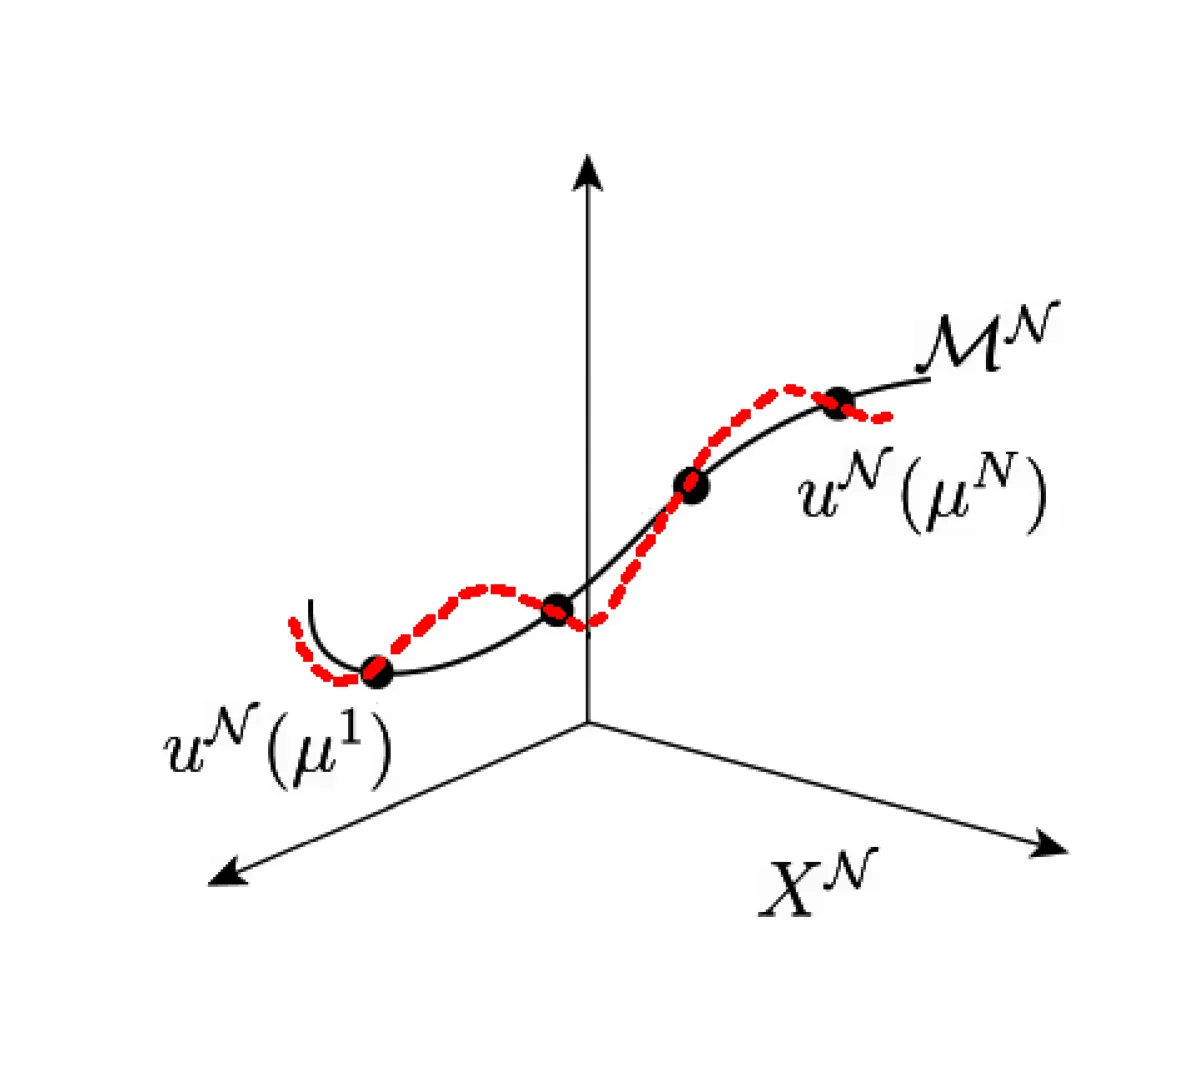
\includegraphics[height=0.8\paperheight]{Manifold.png}
    \end{figure}
\end{frame}

\begin{frame}{Reduced Basis Approximation}
    \begin{block}{}
        Let $\{\xi_n\}_{n=1}^{N}$ denote the reduced basis and define matrix $\mathbf{B} \in \mathbb{R}^{N_{\delta} \times N}$ such that
        $$\xi_n = \sum_{i=1}^{N_{\delta}} \mathbf{B}_{in} \psi_i$$
        i.e., the n-th column of $\mathbf{B}$ denotes the coefficients when the n-th basis function $\xi_n$ is expressed in terms of the basis functions $\{\psi_i\}_{i=1}^{N_{\delta}}$. Then, the reduced basis solution matrix $\mathbf{A}_{rb}^{\mu} \in \mathbb{R}^{N \times N}$ and the right hand side $f_{rb}^{\mu} \in \mathbb{R}^{N}$ defined by 
        $$
        (\mathbf{A}_{rb}^{\mu})_{mn} = a(\xi_n, \xi_m; \mu) \mspace{10mu} \text{and} \mspace{10mu}(f_{rb}^{\mu})_m = f(\xi_m;\mu) \mspace{25mu} 1\leq n,m \leq N
        $$
        can be computed by 
        $$
        \mathbf{A}_{rb}^{\mu} = \mathbf{B}^T \mathbf{A}_{\delta}^{\mu}\mathbf{B} \mspace{10mu} \text{and} \mspace{10mu} f_{rb}^{\mu} = \mathbf{B}^T f_{\delta}^{\mu}
        $$
        
        The reduced basis approximation $u_{rb}^{\mu} = \sum_{n=1}^{N}(u_{rb}^{\mu})_n \xi_n$ is obtained by solving the linear system
        $$
        \mathbf{A}_{rb}^{\mu}u_{rb}^{\mu} = f_{rb}^{\mu}
        $$
        and the output of interest evaluated as $s_{rb}(\mu) = (u_{rb}^{\mu})^T f_{rb}^{\mu}$
    \end{block}
\end{frame}

\begin{frame}{Accuracy}
\begin{block}{}
$$
\|u(\mu) - u_{rb}(\mu)\|_{\mathbb{V}} \leq \|u(\mu) - u_{\delta}(\mu)\|_{\mathbb{V}} + \|u_{\delta}(\mu) - u_{rb}(\mu)\|_{\mathbb{V}}
$$
\end{block}

Applying Cea's lemma for a given approximation space $\mathbb{V}_{rb}$ and a given parameter value $\mu \in \mathbb{P}$, the best approximation error can be connected with the reduced approximation:
$$
\|u(\mu) - u_{rb}(\mu)\|_{\mathbb{V}} \leq \left( 1 + \frac{\gamma(\mu)}{\alpha(\mu)}\right) \inf_{v_{rb} \in \mathbb{V}_{rb}} \|u(\mu) - v_{rb}\|_{\mathbb{V}}
$$
    
\end{frame}

\begin{frame}{Reduced Basis Model}
    \begin{figure}
        \centering
        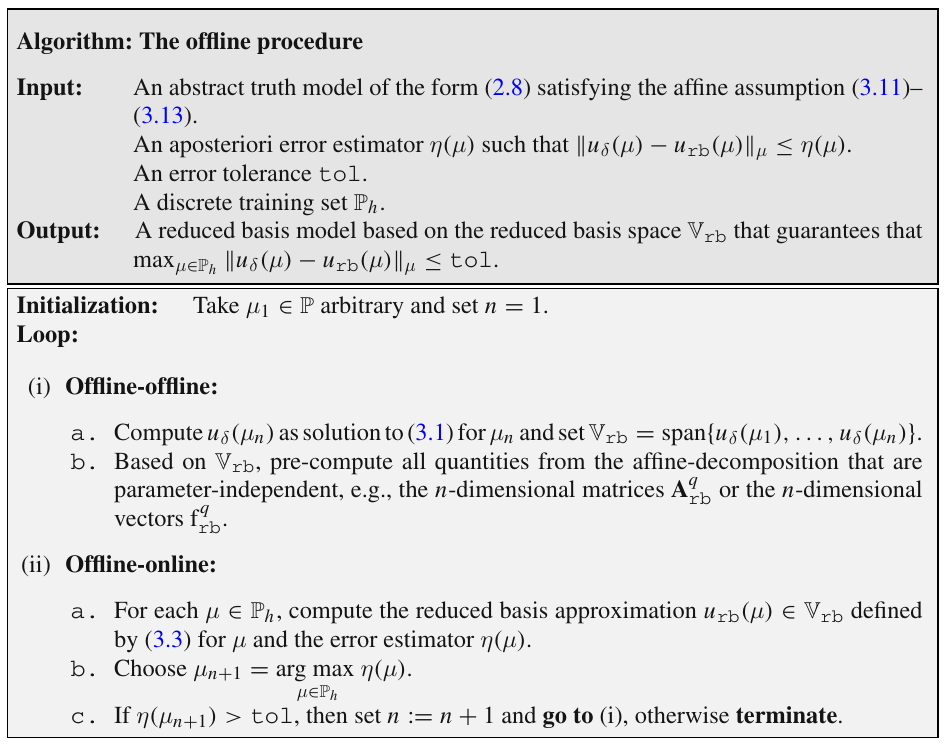
\includegraphics[height=0.75\paperheight]{Offline.png}
    \end{figure}
\end{frame}

\begin{frame}{Reduced Basis Model}
    \begin{figure}
        \centering
        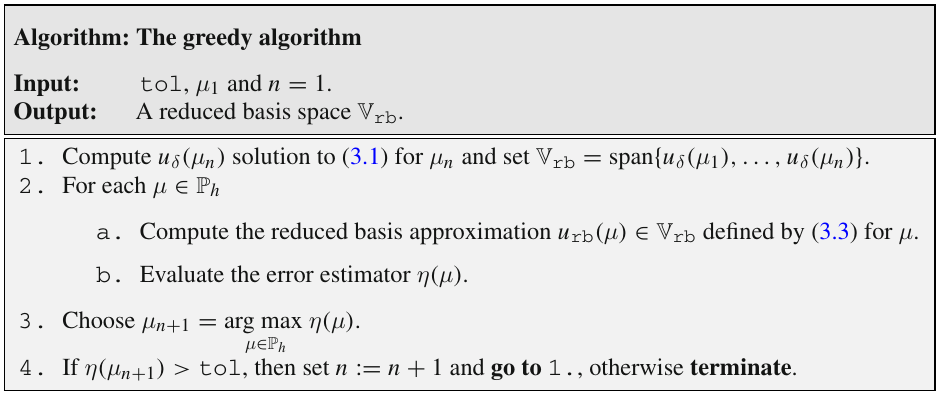
\includegraphics[width=\textwidth]{Greedy.png}
    \end{figure}
\end{frame}

\begin{frame}{Reduced Basis Model}
    \begin{figure}
        \centering
        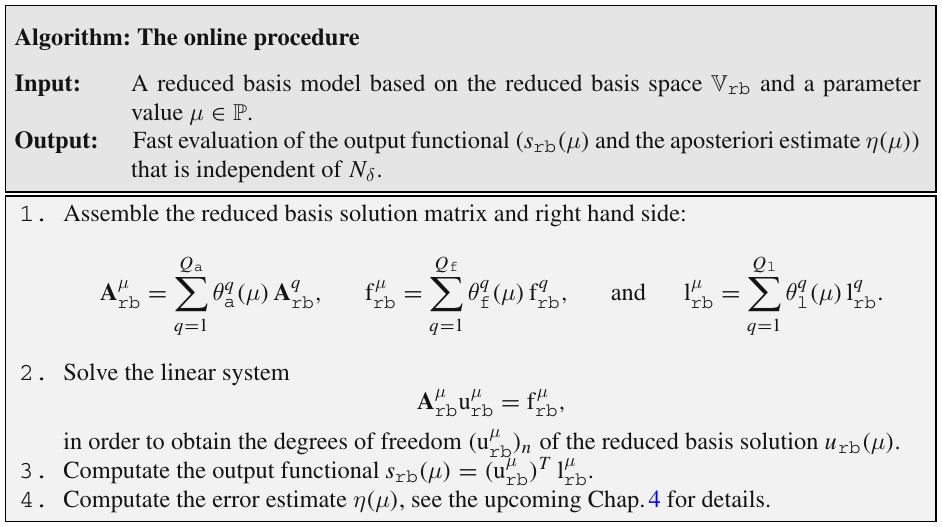
\includegraphics[width=\textwidth]{Online.png}
    \end{figure}
\end{frame}

\begin{frame}{Orders of Complexity}
\begin{enumerate}
    \item Offline
    $$\mathcal{O}(NN_{\delta}^p) \mspace{25mu} p \leq 3$$
    
    \item Online
    \begin{itemize}
        \item Assembling Operators
        $$\mathcal{O}(Q_a N^2)$$
        $$\mathcal{O}(Q_f N)$$
        $$\mathcal{O}(Q_l N)$$
        
        \item Recover RB solution
        $$\mathcal{O}(N^3)$$
    \end{itemize}
\end{enumerate}
\end{frame}



\section[Thermal Block]{Heat Conduction} 
\begin{frame}{Thermal Block Problem}
    Consider steady heat conduction in a two-dimensional domain:
    \begin{figure}
        \centering
        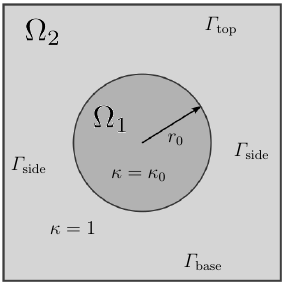
\includegraphics[width=0.35\textwidth]{thermal_block.png}
    \end{figure}
    We define two subdomains $\Omega_1$ and $\Omega_2$, such that
 \begin{enumerate}
 \item $\Omega_1$ is a disk centered at the origin of radius $r_0=0.5$, and
 \item $\Omega_2=\Omega/\ \overline{\Omega_1}$.
 \end{enumerate}
\end{frame}

\begin{frame}{Thermal Block Problem}
\begin{figure}
        \centering
        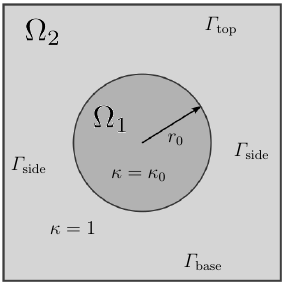
\includegraphics[width=0.25\textwidth]{thermal_block.png}
    \end{figure}
\begin{block}{}
    The conductivity $\kappa$ is assumed to be constant on $\Omega_1$ and $\Omega_2$, i.e.
$$
\kappa|_{\Omega_1}=\kappa_0 \quad \textrm{and} \quad \kappa|_{\Omega_2}=1.
$$
\end{block}

\begin{block}{}
  For this problem, we consider $P=2$ parameters:
\begin{enumerate}
\item the first one is related to the conductivity in $\Omega_1$, i.e. $\mu_0\equiv k_0$;
\item the second parameter $\mu_1$ takes into account the constant heat flux over $\Gamma_{base}$.
\end{enumerate}

The parameter vector $\boldsymbol{\mu}$ is thus given by 
$
\boldsymbol{\mu} = (\mu_0,\mu_1)
$
on the parameter domain
$
\mathbb{P}=[0.1,10]\times[-1,1].
$
\end{block}
\end{frame}

\begin{frame}{Thermal Block Problem}
\begin{block}{}
    \begin{figure}
        \centering
        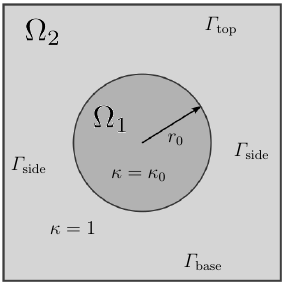
\includegraphics[width=0.35\textwidth]{thermal_block.png}
    \end{figure}
Model the heat transfer process due to the heat flux over the bottom boundary $\Gamma_{base}$ and the following conditions on the remaining boundaries:
\begin{itemize}
    \item the left and right boundaries $\Gamma_{side}$ are insulated,
    \item the top boundary $\Gamma_{top}$ is kept at a reference temperature (say, zero),
\end{itemize}
with the aim of measuring the average temperature on $\Gamma_{base}$.
\end{block}
\end{frame}


\begin{frame}{Parametrised Formulation}
\begin{exampleblock}{}
For a given parameter $\boldsymbol{\mu}\in\mathbb{P}$, find $u(\boldsymbol{\mu})$ such that
$$
\begin{cases}
	- \text{div} (\kappa(\mu_0)\nabla u(\boldsymbol{\mu})) = 0 & \text{in } \Omega,\\
	u(\boldsymbol{\mu}) = 0 & \text{on } \Gamma_{top},\\
	\kappa(\mu_0)\nabla u(\boldsymbol{\mu})\cdot \mathbf{n} = 0 & \text{on } \Gamma_{side},\\
	\kappa(\mu_0)\nabla u(\boldsymbol{\mu})\cdot \mathbf{n} = \mu_1 & \text{on } \Gamma_{base}.
\end{cases}
$$
\end{exampleblock}

\begin{block}{}
\begin{itemize}
    \item $\mathbf{n}$ denotes the outer normal to the boundaries $\Gamma_{side}$ and $\Gamma_{base}$,
    \item the conductivity $\kappa(\mu_0)$ is defined as follows:
    $$
\kappa(\mu_0) =
\begin{cases}
	\mu_0 & \text{in } \Omega_1,\\
	1 & \text{in } \Omega_2,\\
\end{cases}
$$
\end{itemize}
\end{block}
\end{frame}

\begin{frame}{Weak Formulation}
\begin{exampleblock}{}
For a given parameter $\boldsymbol{\mu}\in\mathbb{P}$, find $u(\boldsymbol{\mu})\in\mathbb{V}$ such that
$$a\left(u(\boldsymbol{\mu}),v;\boldsymbol{\mu}\right)=f(v;\boldsymbol{\mu})\quad \forall v\in\mathbb{V}$$
\end{exampleblock}

\begin{block}{}
\begin{enumerate}
    \item functional space $\mathbb{V}$:
$$
\mathbb{V} = \{v\in H^1(\Omega) : v|_{\Gamma_{top}}=0\}
$$
    \item parametrised bilinear form $a(\cdot, \cdot; \boldsymbol{\mu}): \mathbb{V} \times \mathbb{V} \to \mathbb{R}$:
$$a(u, v;\boldsymbol{\mu})=\int_{\Omega} \kappa(\mu_0)\nabla u\cdot \nabla v \ d\boldsymbol{x},$$
    \item parametrised linear form $f(\cdot; \boldsymbol{\mu}): \mathbb{V} \to \mathbb{R}$:
$$f(v; \boldsymbol{\mu})= \mu_1\int_{\Gamma_{base}}v \ ds.$$
\end{enumerate}
\end{block}
\end{frame}

\begin{frame}{Weak Formulation}
\begin{exampleblock}{}
For a given parameter $\boldsymbol{\mu}\in\mathbb{P}$, find $u(\boldsymbol{\mu})\in\mathbb{V}$ such that
$$a\left(u(\boldsymbol{\mu}),v;\boldsymbol{\mu}\right)=f(v;\boldsymbol{\mu})\quad \forall v\in\mathbb{V}$$
\end{exampleblock}

\begin{alertblock}{}
The output of interest $s(\boldsymbol{\mu})$ given by
$$s(\boldsymbol{\mu}) = \mu_1\int_{\Gamma_{base}} u(\boldsymbol{\mu})$$
is computed for each $\boldsymbol{\mu}$.
\end{alertblock}
\end{frame}

\begin{frame}{Affine Decomposition}
    \begin{exampleblock}{}
        \begin{equation*}
            \mathrm{a}\left ({u},{v}; \mathbf{\mu} \right ) = \sum_{q=1}^{Q_a} \Theta_q^a (\mu) \mathrm{a}_q\left ({u},{v}\right )
        \end{equation*}
        \begin{equation*}
            \mathrm{f}\left(v;\mu \right) = \sum_{q=1}^{Q_f} \Theta_q^f (\mu) \mathrm{f}_q\left(v \right)
        \end{equation*}
    \end{exampleblock}
    For this problem the affine decomposition is straightforward.
    \begin{exampleblock}{}
        $$a(u,v;\boldsymbol{\mu})=\underbrace{\mu_0}_{\Theta^{a}_0(\boldsymbol{\mu})}\underbrace{\int_{\Omega_1}\nabla u \cdot \nabla v \ d\boldsymbol{x}}_{a_0(u,v)} \ + \  \underbrace{1}_{\Theta^{a}_1(\boldsymbol{\mu})}\underbrace{\int_{\Omega_2}\nabla u \cdot \nabla v \ d\boldsymbol{x}}_{a_1(u,v)},$$
$$f(v; \boldsymbol{\mu}) = \underbrace{\mu_1}_{\Theta^{f}_0(\boldsymbol{\mu})} \underbrace{\int_{\Gamma_{base}}v \ ds}_{f_0(v)}.$$
    \end{exampleblock}

\end{frame}

\begin{frame}{Result - Error}
$$\max_{\mu \in \mathbb{P}_h} \|u_{\delta}(\mu) - u_{rb}(\mu)\|$$
$$\frac{1}{|\mathbb{P}_h|} \sum_{\mu \in \mathbb{P}_h} \|u_{\delta}(\mu) - u_{rb}(\mu)\|$$
\begin{figure}
    \centering
    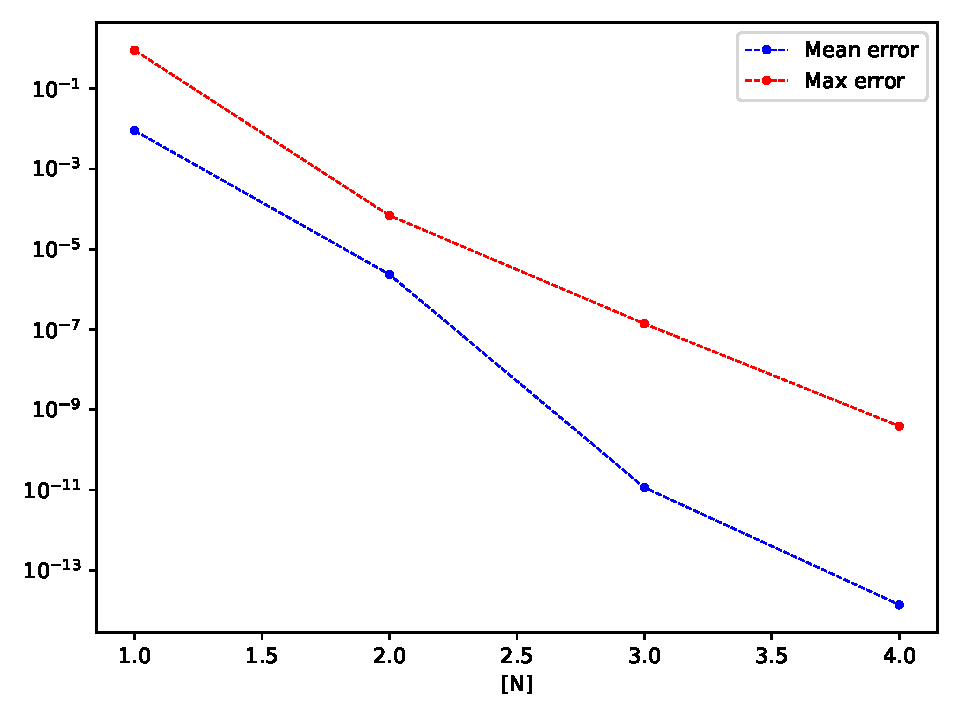
\includegraphics[height=0.55\paperheight]{output_error.pdf}
\end{figure}
\end{frame}

\begin{frame}{Result - Speedup}

\begin{figure}
    \centering
    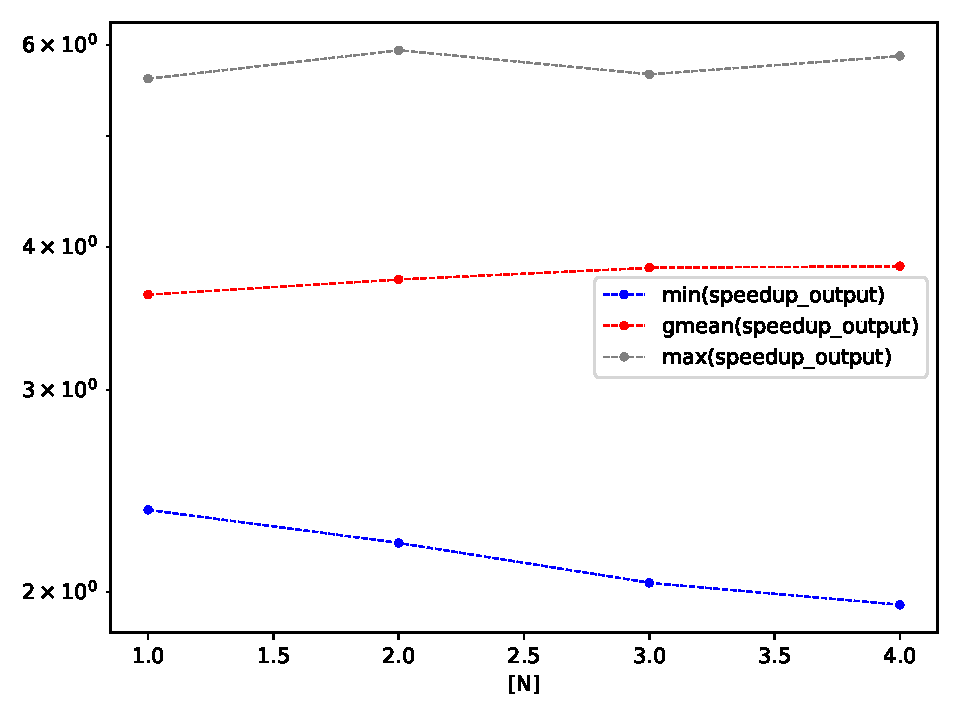
\includegraphics[height=0.75\paperheight]{speedup_output.pdf}
\end{figure}
\end{frame}

\section[Navier Stokes]{Fluid Flow} 
\begin{frame}{Navier Stokes}

Navier-Stokes equations over the two-dimensional backward-facing step domain $\Omega$ shown below:

\begin{figure}
    \centering
    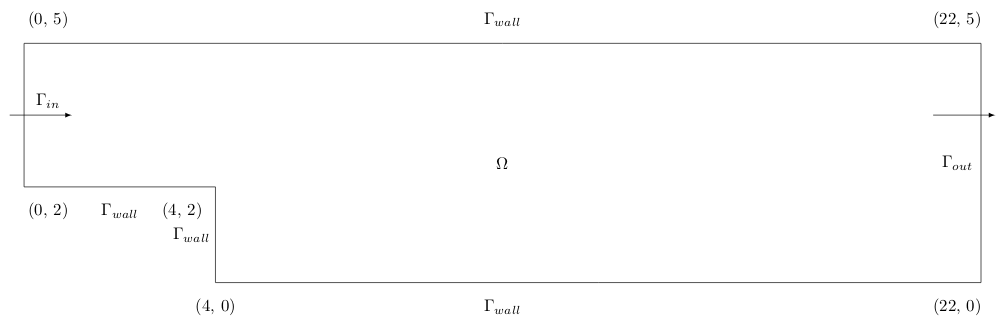
\includegraphics[width=0.5\textwidth]{channel.png}

\end{figure}

A Poiseuille flow profile is imposed on the inlet boundary, and a no-flow (zero velocity) condition is imposed on the walls. A homogeneous Neumann condition of the Cauchy stress tensor is applied at the outflow boundary.

The inflow velocity boundary condition is characterized by $$\boldsymbol{u}(\boldsymbol{x};\mu)=\mu\bigg \{\frac{1}{2.25}(x_1-2)(5-x_1),0\bigg \} \quad \forall \boldsymbol{x}=(x_0,x_1) \in \Omega$$ 

This problem is characterized by one parameter $\mu$, which characterizes the inlet velocity. The range of $\mu$ is the following $$\mu \in [1.0, 80.0].$$ 

Thus, the parameter domain is $$\mathbb{P}=[1.0,80.0].$$

\end{frame}

\begin{frame}{Result - Error Velocity}
$$\max_{\mu \in \mathbb{P}_h} \|u_{\delta}(\mu) - u_{rb}(\mu)\|$$
$$\frac{1}{|\mathbb{P}_h|} \sum_{\mu \in \mathbb{P}_h} \|u_{\delta}(\mu) - u_{rb}(\mu)\|$$
\begin{figure}
    \centering
    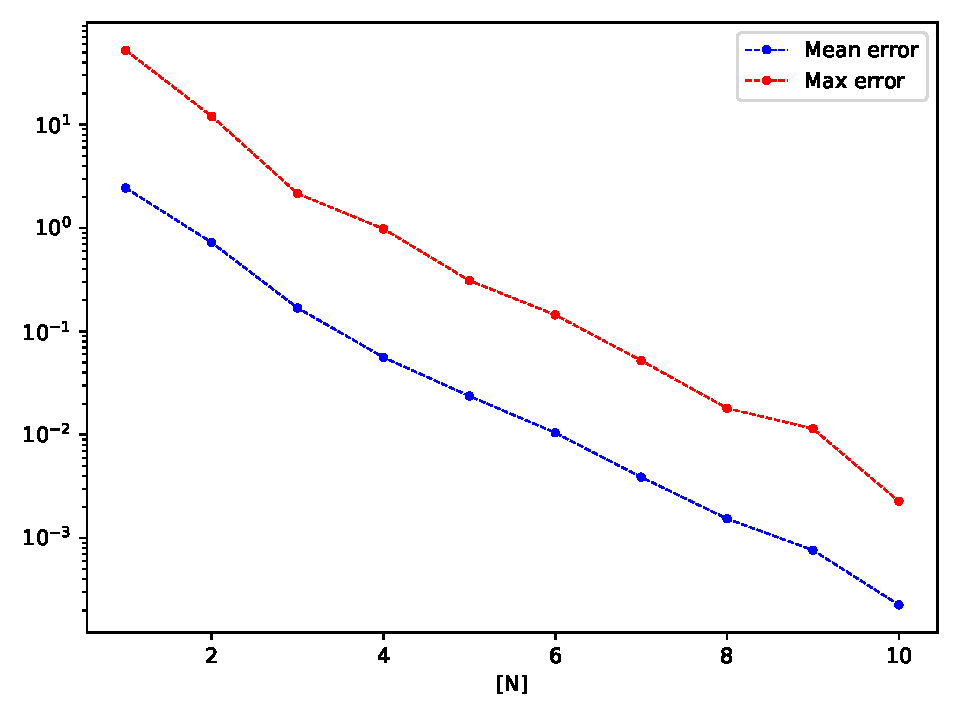
\includegraphics[height=0.55\paperheight]{output_error_u.pdf}
\end{figure}
\end{frame}

\begin{frame}{Result - Error Pressure}
$$\max_{\mu \in \mathbb{P}_h} \|u_{\delta}(\mu) - u_{rb}(\mu)\|$$
$$\frac{1}{|\mathbb{P}_h|} \sum_{\mu \in \mathbb{P}_h} \|u_{\delta}(\mu) - u_{rb}(\mu)\|$$
\begin{figure}
    \centering
    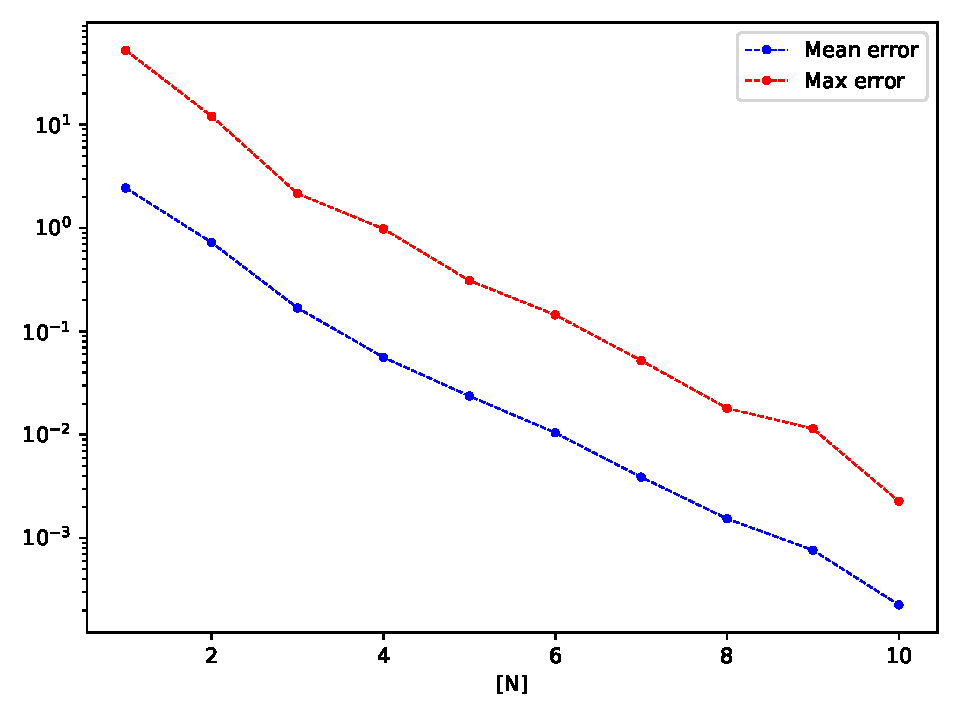
\includegraphics[height=0.55\paperheight]{output_error_p.pdf}
\end{figure}
\end{frame}

\begin{frame}{Result - Speedup}

\begin{figure}
    \centering
    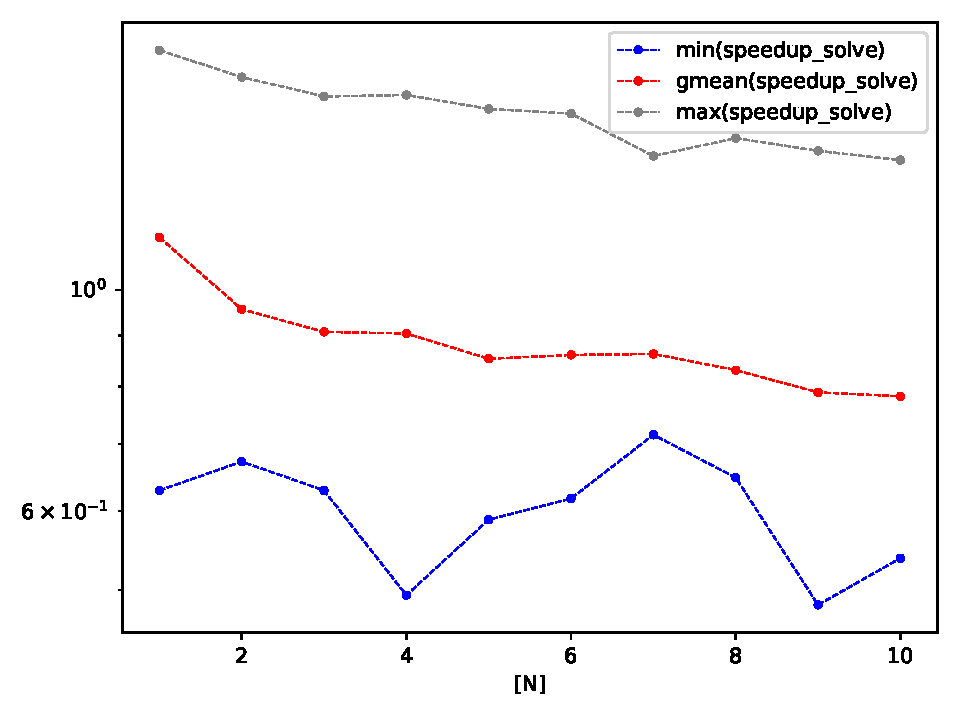
\includegraphics[height=0.75\paperheight]{speedup_solve.pdf}
\end{figure}
\end{frame}
 
\end{document}